% --------------------------------------------------------------------------- %
% --------------------------------------------------------------------------- %
\section{Multijet Estimate}
\label{sec:qcd}

The estimate of the SM multijet background utilizes two different techniques depending on the number of jets in a given signal region. For regions with two or more jets, the background is estimated by extrapolating to regions with high \dphimin after inverting the \dphimin requirement. In the monojet signal regions, a sample enriched in unbalanced dijet events is used to extrapolate to regions with low sub-leading jet momentum.

\subsection{Multijet Signal Region Prediction}
\label{subsec:qcdMultijet}

As outlined in section \ref{subsec:multijetCR}, the multijet background in control regions with two or more jets is estimated using a QCD-enriched sample where \HT triggers are used to select events with an inverted \dphimin cut. The ratio of events with high to low \dphimin (\rphi) is modeled as a power law function in \mttwo, as shown in equation \ref{eq:rphi}. 
\begin{equation}
	r_{\phi}(\mttwomath) = \frac{N(\dphiminmath > 0.3)}{N(\dphiminmath < 0.3)} = a \cdot M_{\mathrm{T2}}^b
	\label{eq:rphi}
\end{equation}

The power-law dependence of \rphi on \mttwo is verified in simulation for events with $\mttwomath > 60 \GeV$,, as illustrated in figure \ref{fig:rphiDependence}. Because the dominant source of \MET in low \mttwo events is not necessarily due to jet mismeasurement, the fit is performed in the window $60 < \mttwomath < 100 \GeV$ except in extreme \HT regions where a lower bound of 70\GeV is used (as a conservative measure since these regions have high statistics). The upper bound of 100 \GeV is chosen such that the contamination of electroweak and top-quark events is small compared to the QCD multijet yield. A systematic uncertainty in the \rphi value is assigned based on variations of the fit window, by shifting the lower boundary of the window in either direction while preserving the fit statistics by shifting the upper boundary of the window. The systematic uncertainty is then taken as the maximal deviation of all such variation with respect to the nominal window.
\begin{figure}
	\centering
	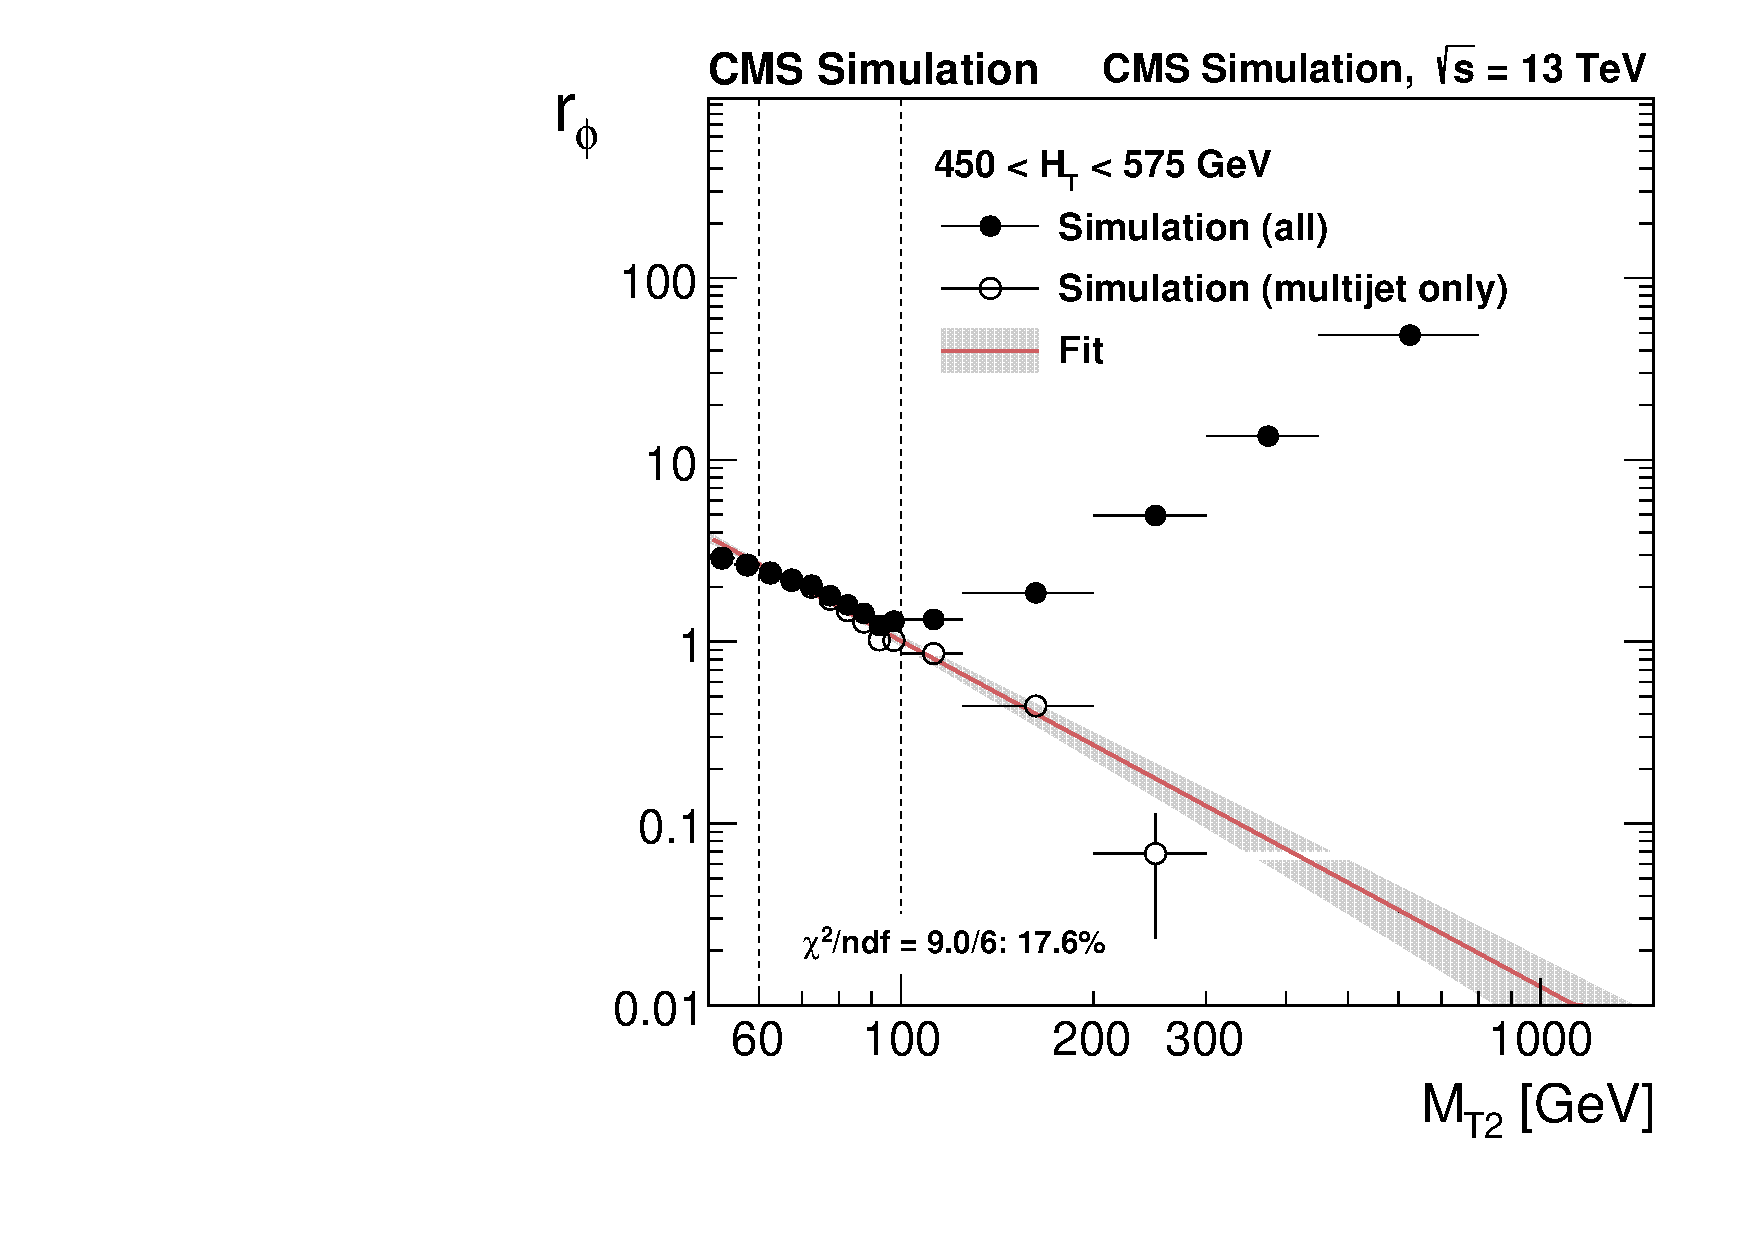
\includegraphics[width=0.35\textwidth]{backgrounds/figs/ratio_HT450to575_j2toInf_b0toInf}
	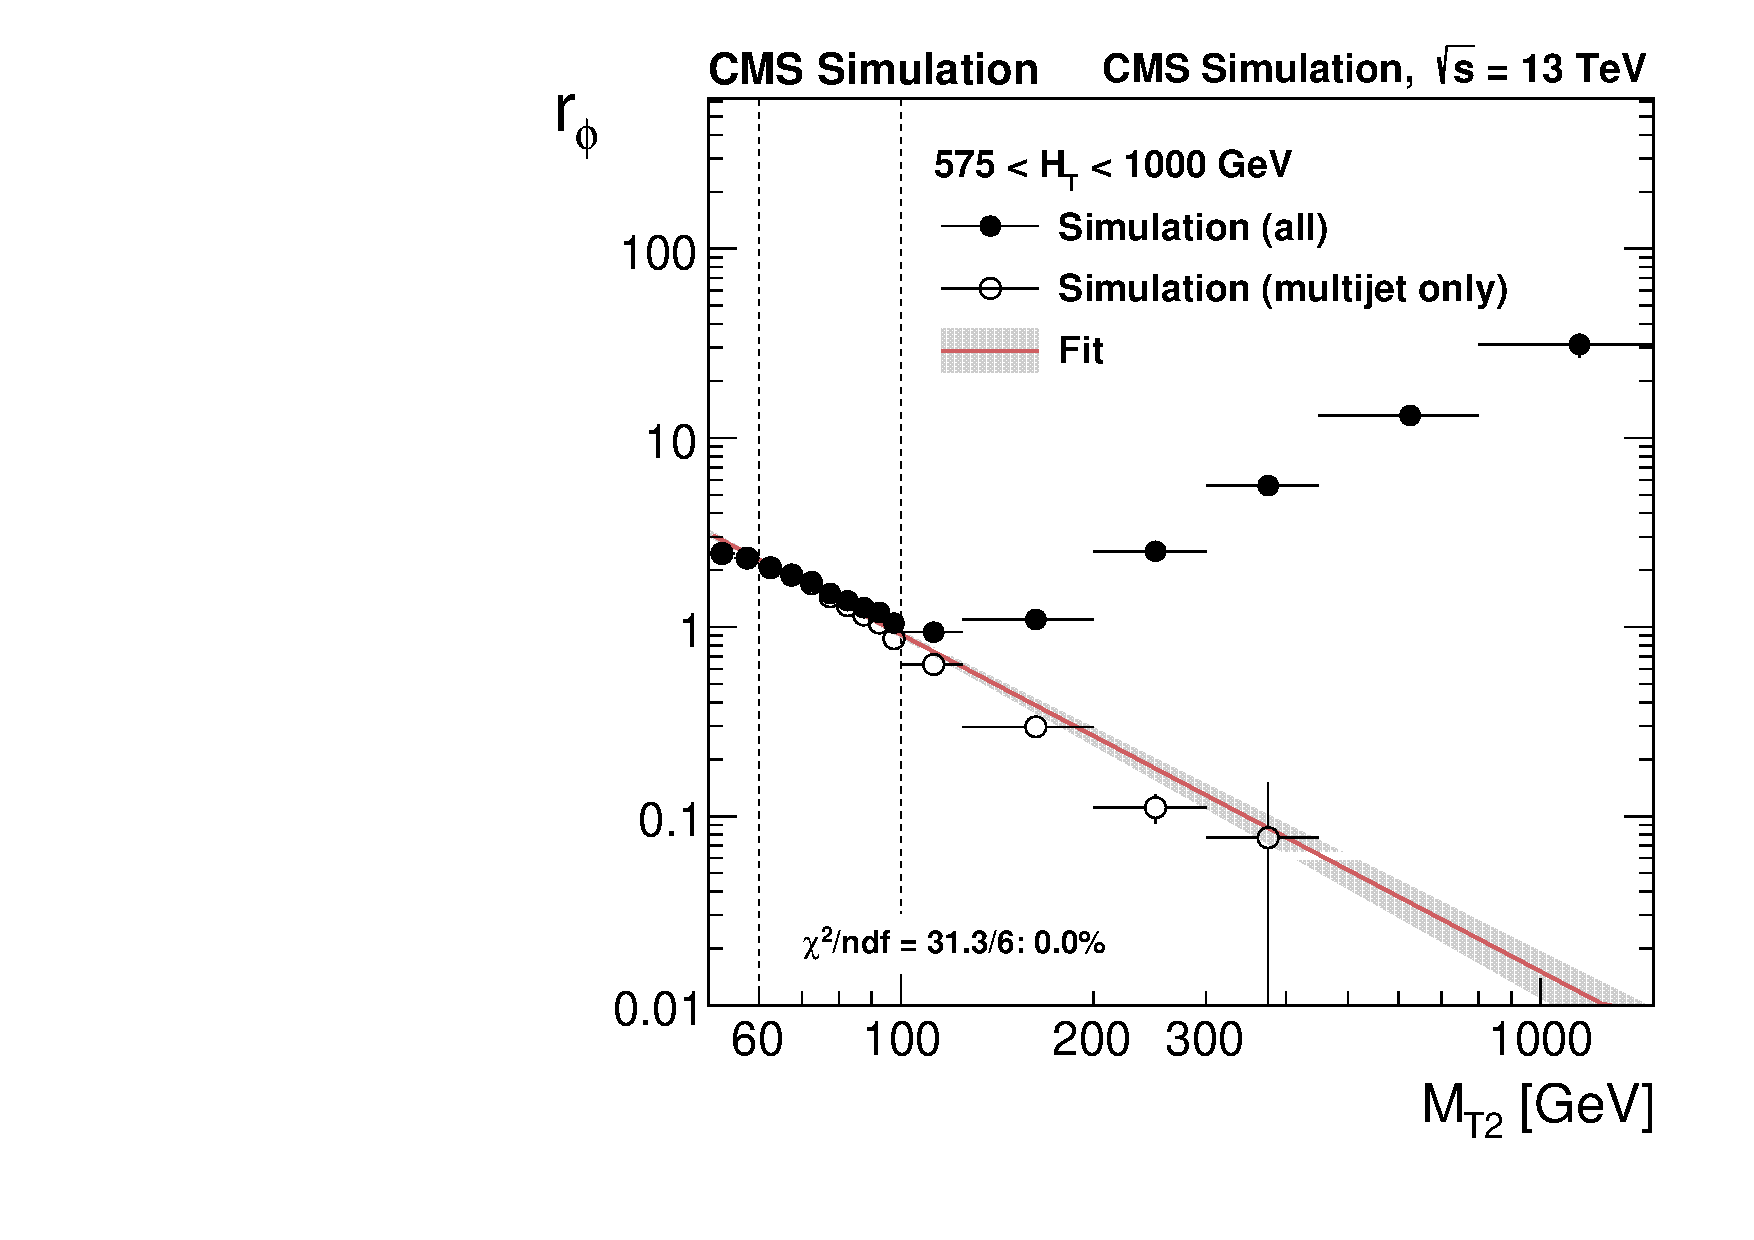
\includegraphics[width=0.35\textwidth]{backgrounds/figs/ratio_HT575to1000_j2toInf_b0toInf}
	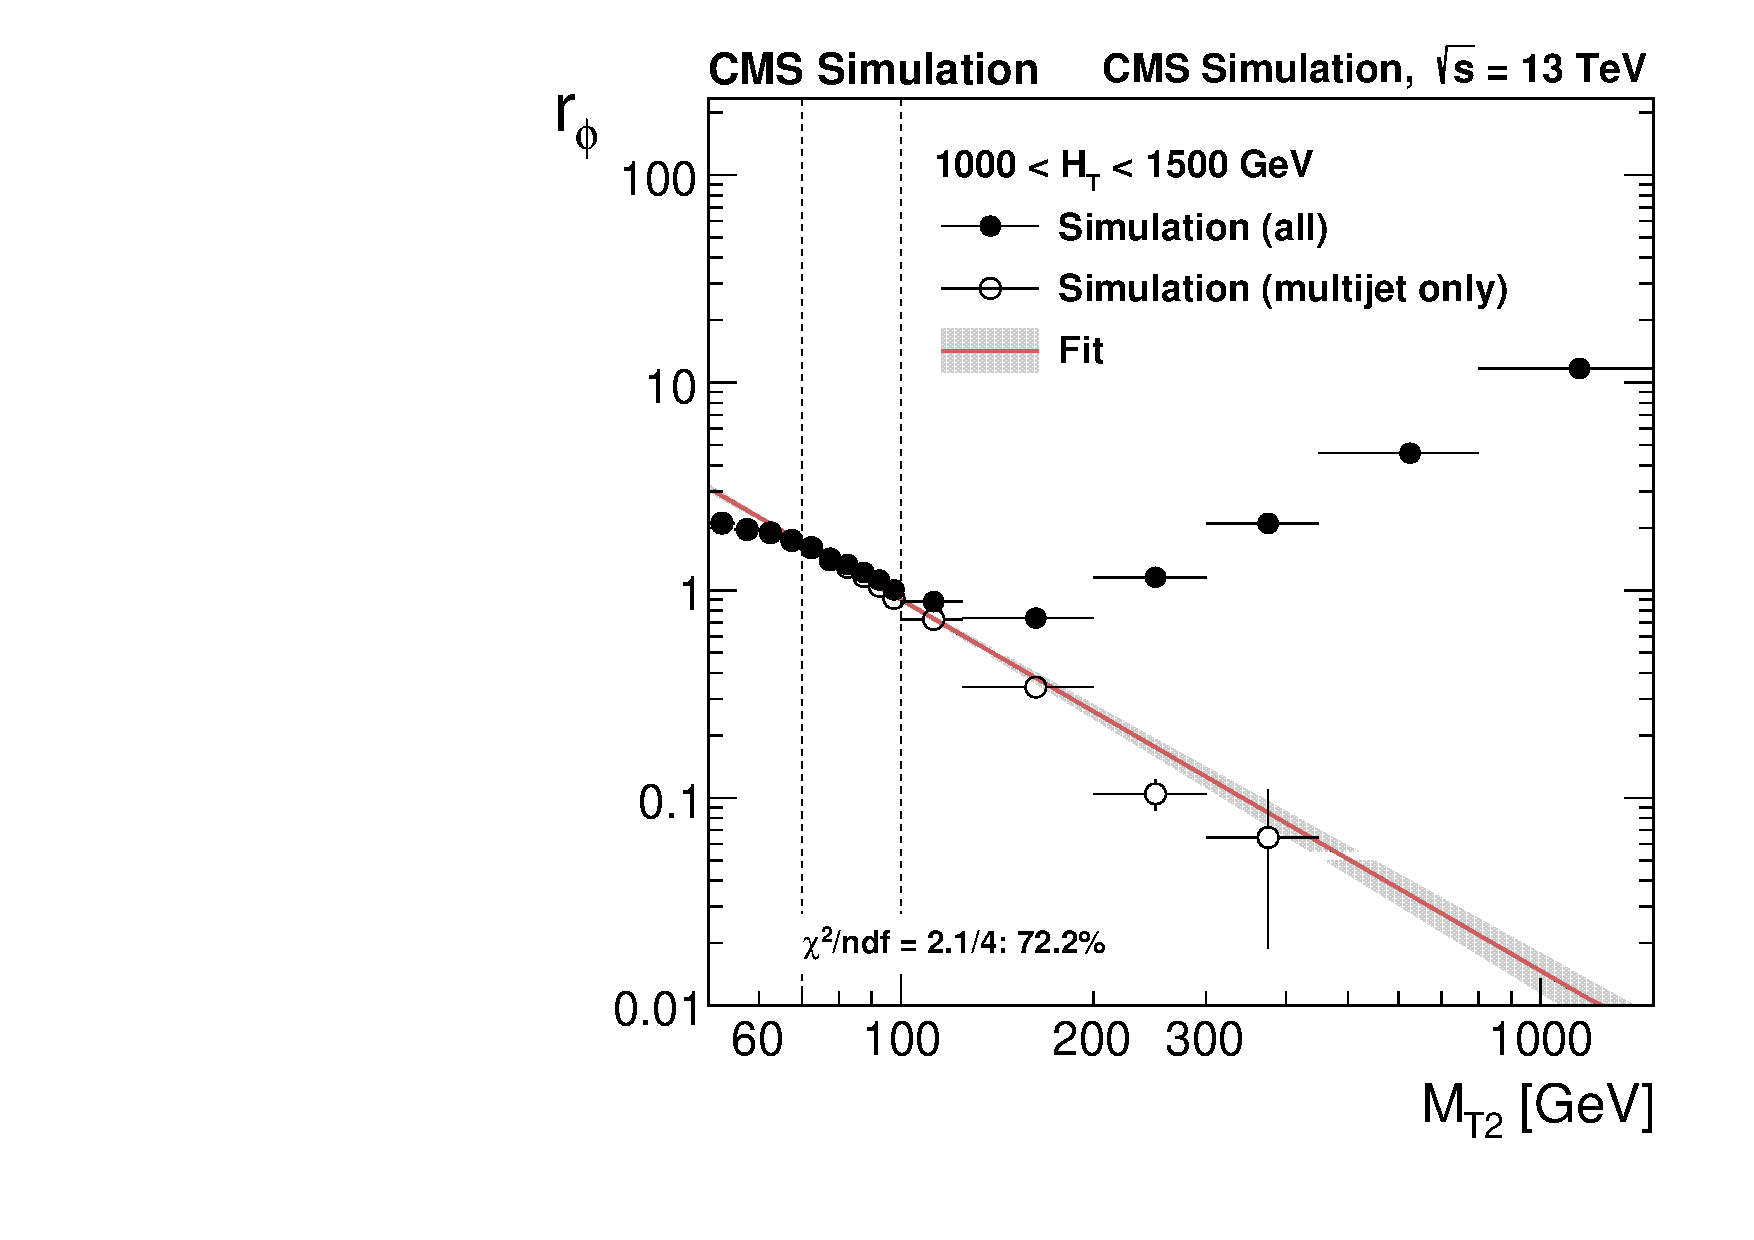
\includegraphics[width=0.35\textwidth]{backgrounds/figs/ratio_HT1000to1500_j2toInf_b0toInf}
	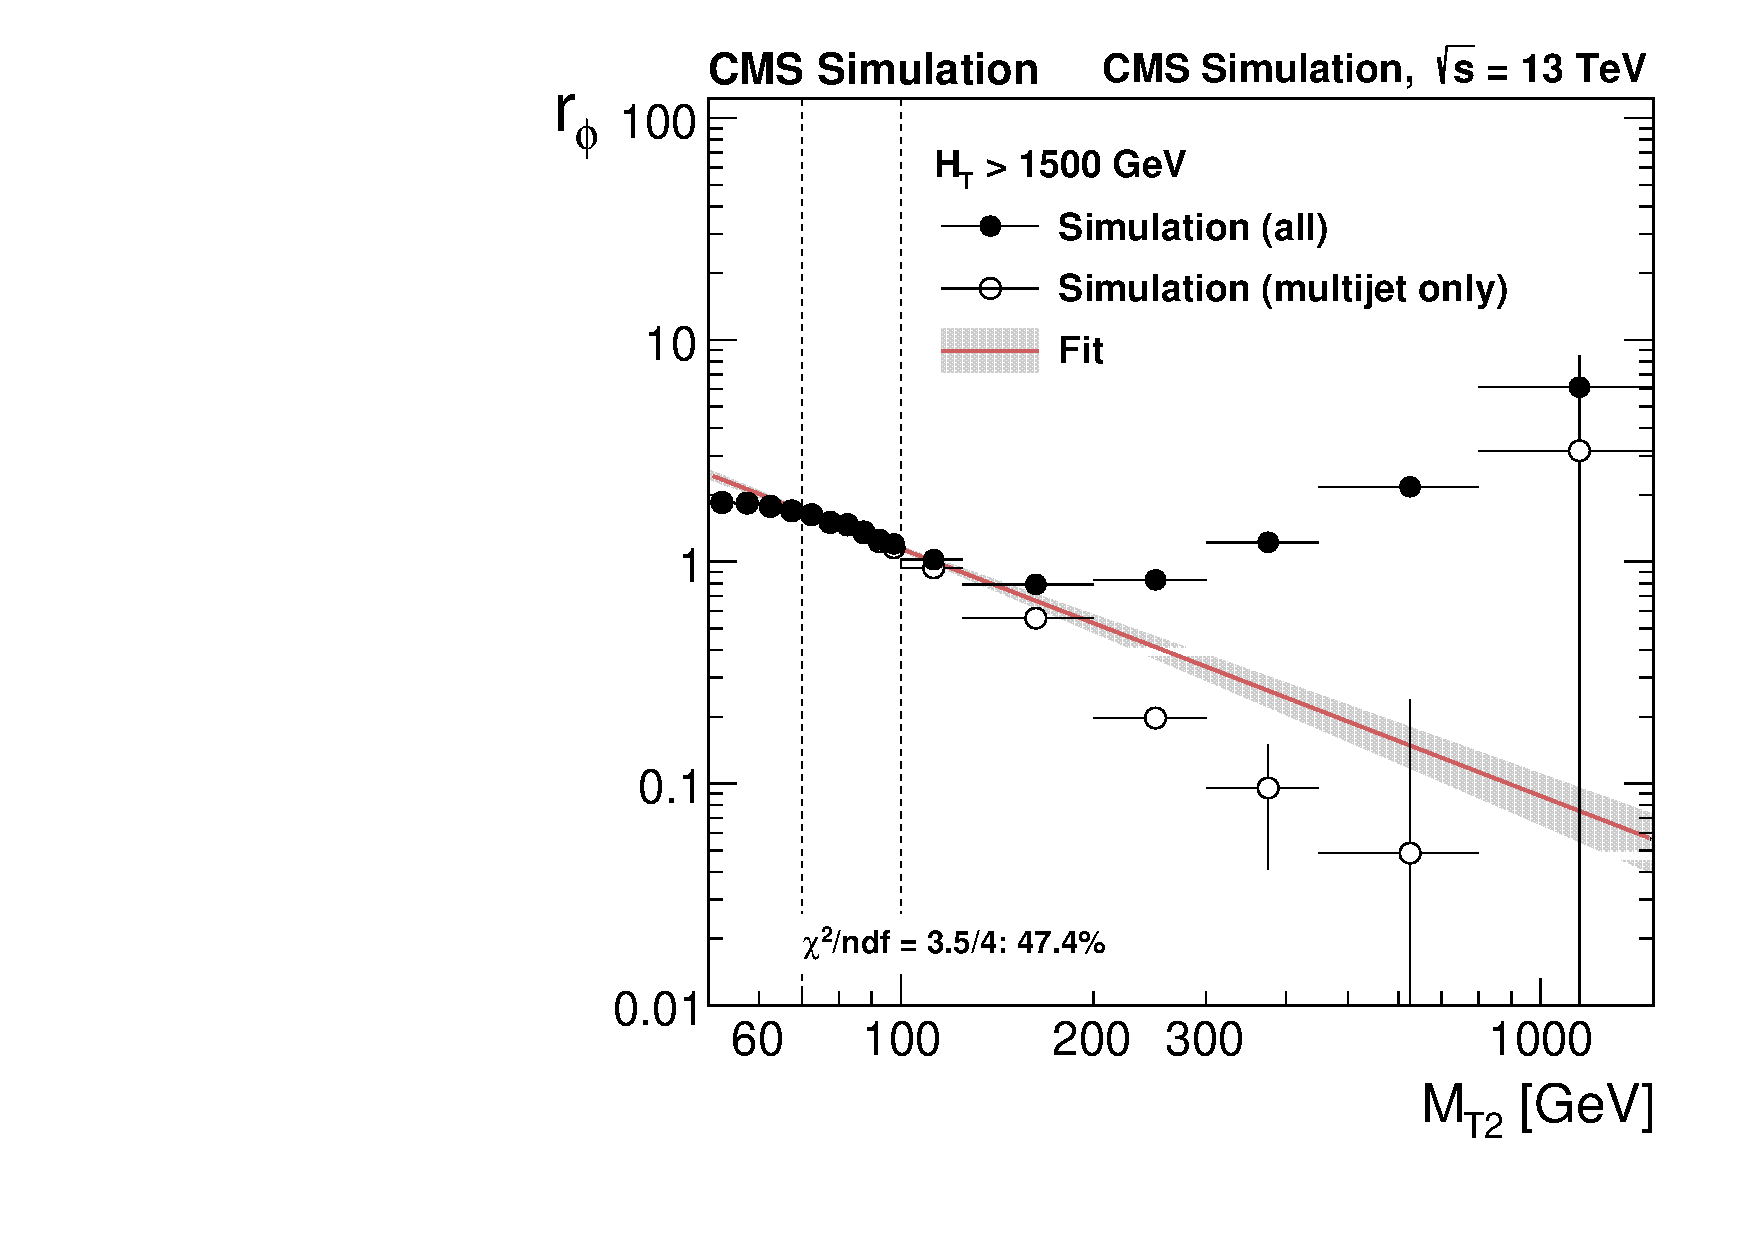
\includegraphics[width=0.35\textwidth]{backgrounds/figs/ratio_HT1500toInf_j2toInf_b0toInf}
	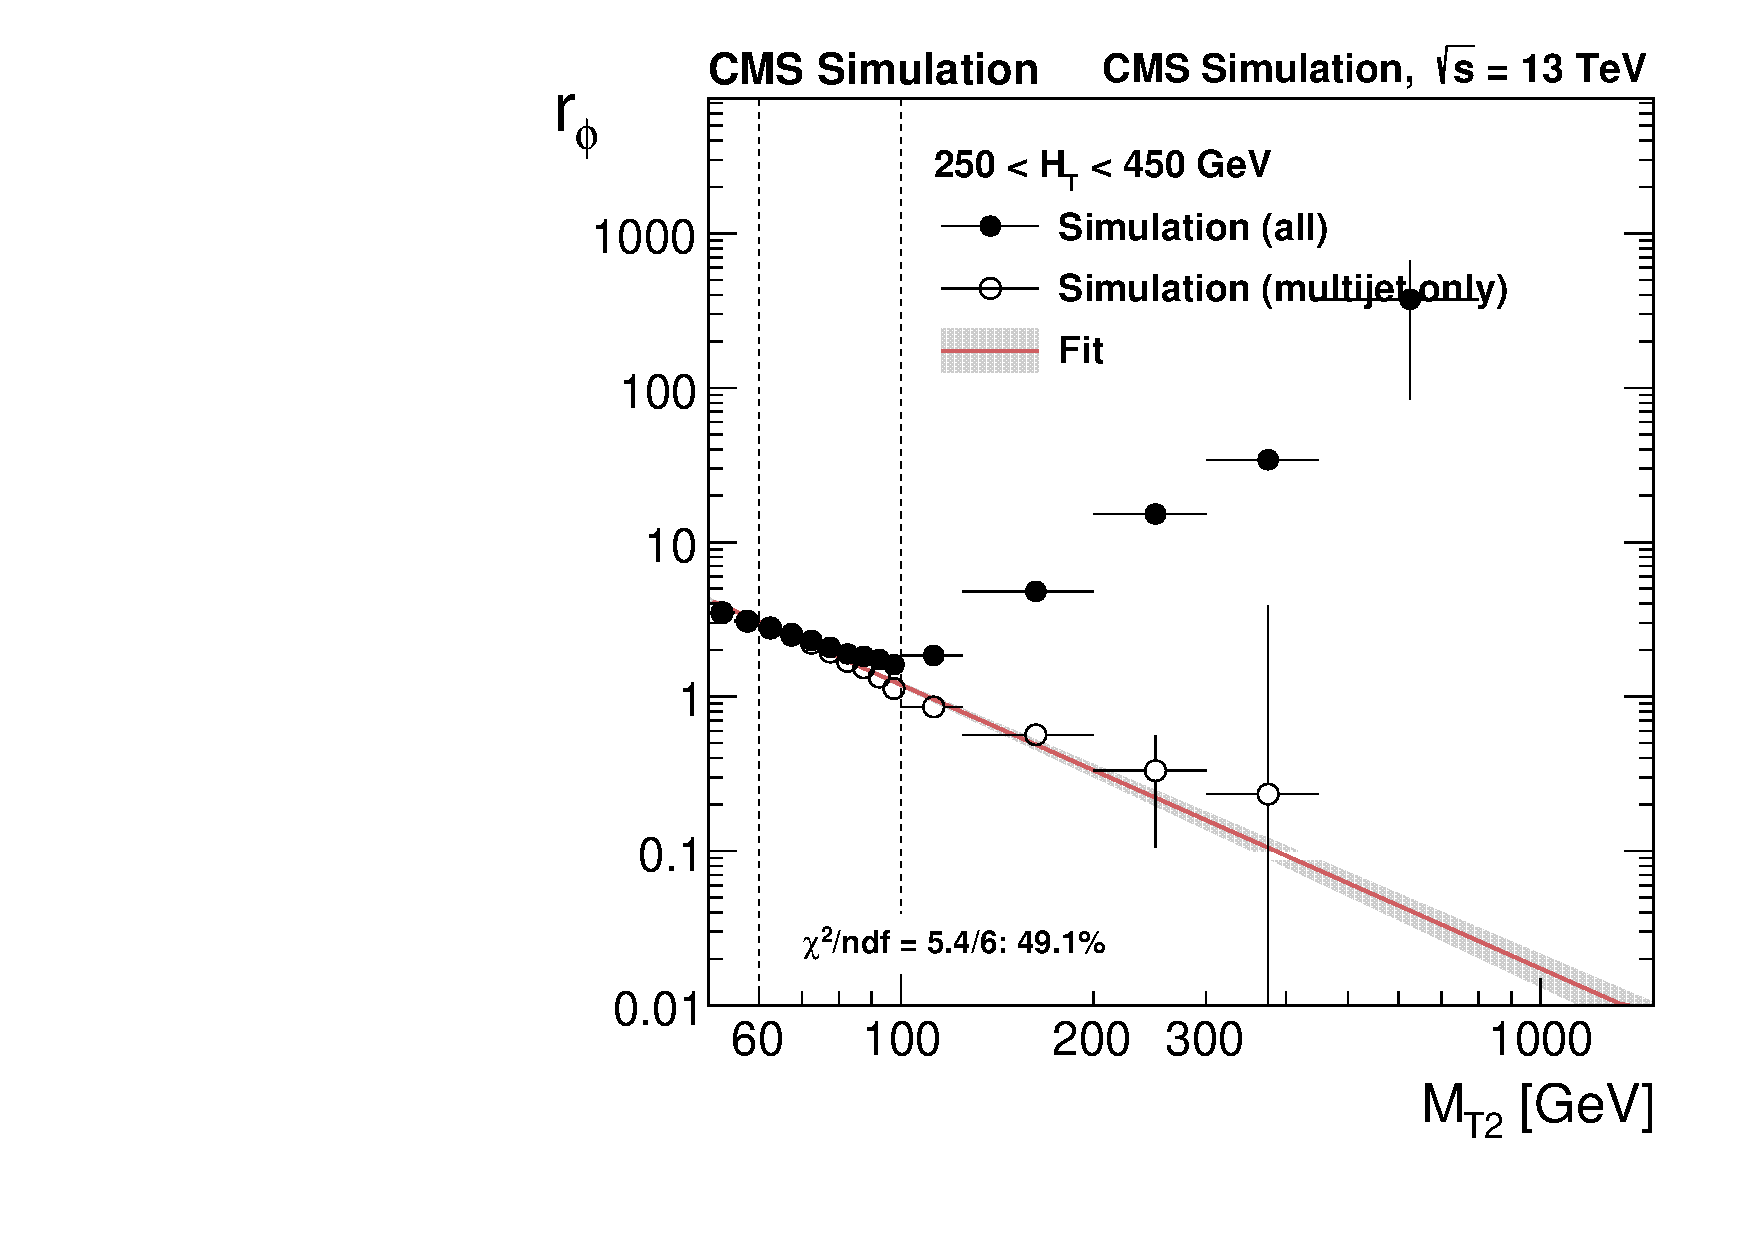
\includegraphics[width=0.35\textwidth]{backgrounds/figs/ratio_HT250to450_j2toInf_b0toInf}
	\caption{Simulated distribution of the \rphi ratio as a function of \mttwo for the low (top left), medium (top right), high (medium left), extreme (medium right), and very low (bottom) \HT regions. Solid points represent the total simulated background, and hollow points show the QCD multijet contribution only. The red line and grey error band illustrates the best fit to a power law function performed in the dashed line fit window}
	\label{fig:rphiDependence}
\end{figure}

Due to the the total integrated luminosity available and the deliberate suppression rate with which some \HT triggers save events (known as the trigger {\it prescale}), the statistics are sufficient to perform fits in \HT regions inclusive in \nj and \nj. The inclusive multijet background estimate can be determined using \rphi as a function of \mttwo $N_{\mathrm{inc}}^{SR} = r_\phi (\mttwomath) \cdot N_{\mathrm{inc}}^{CR} (\mttwomath)$. The final estimate in a given \nj-\nb bin can be determined as in equation \ref{eq:qcdEstimate}, where \fj is the fraction of multijet events in bin \nj in a given \HT bin, and \rb is the ratio of events with \nb b-tags in a given \nj bin. 
\begin{equation}
	N_{j,b}^{SR}(\mttwomath) = r_\phi (\mttwomath) \cdot N_{\mathrm{inc}}^{CR} (\mttwomath) \cdot f_j (H_{\mathrm{T}}) \cdot r_b (N_{\mathrm{jets}}) 
	\label{eq:qcdEstimate}
\end{equation}

The values of \fj and \rb are measured in data using QCD-enriched regions with an inverted \dphi requirement and $100 < \mttwomath < 200$. Based on simulation, \fj and \rb do not significantly depend on \mttwo, and \rb is independent of \HT. Since \fj is dependent on \HT and \rb on \nj, different values of \fj are measured in each inclusive \HT region, and different values of \rb are measured in in inclusive \nj regions. Figures \ref{fig:fj} and \ref{fig:rb} illustrates the data-driven values of \fj and \rb respectively, along with a comparison to simulation. The robustness of invariance with respect to \mttwo and \dphi (and \HT for \rb) is calculated by making several variations of the aforementioned variables and measuring consequent variations in \fj and \rb, and is summarized in table \ref{tbl:fjrbSyst}.

\begin{figure}
	\centering
	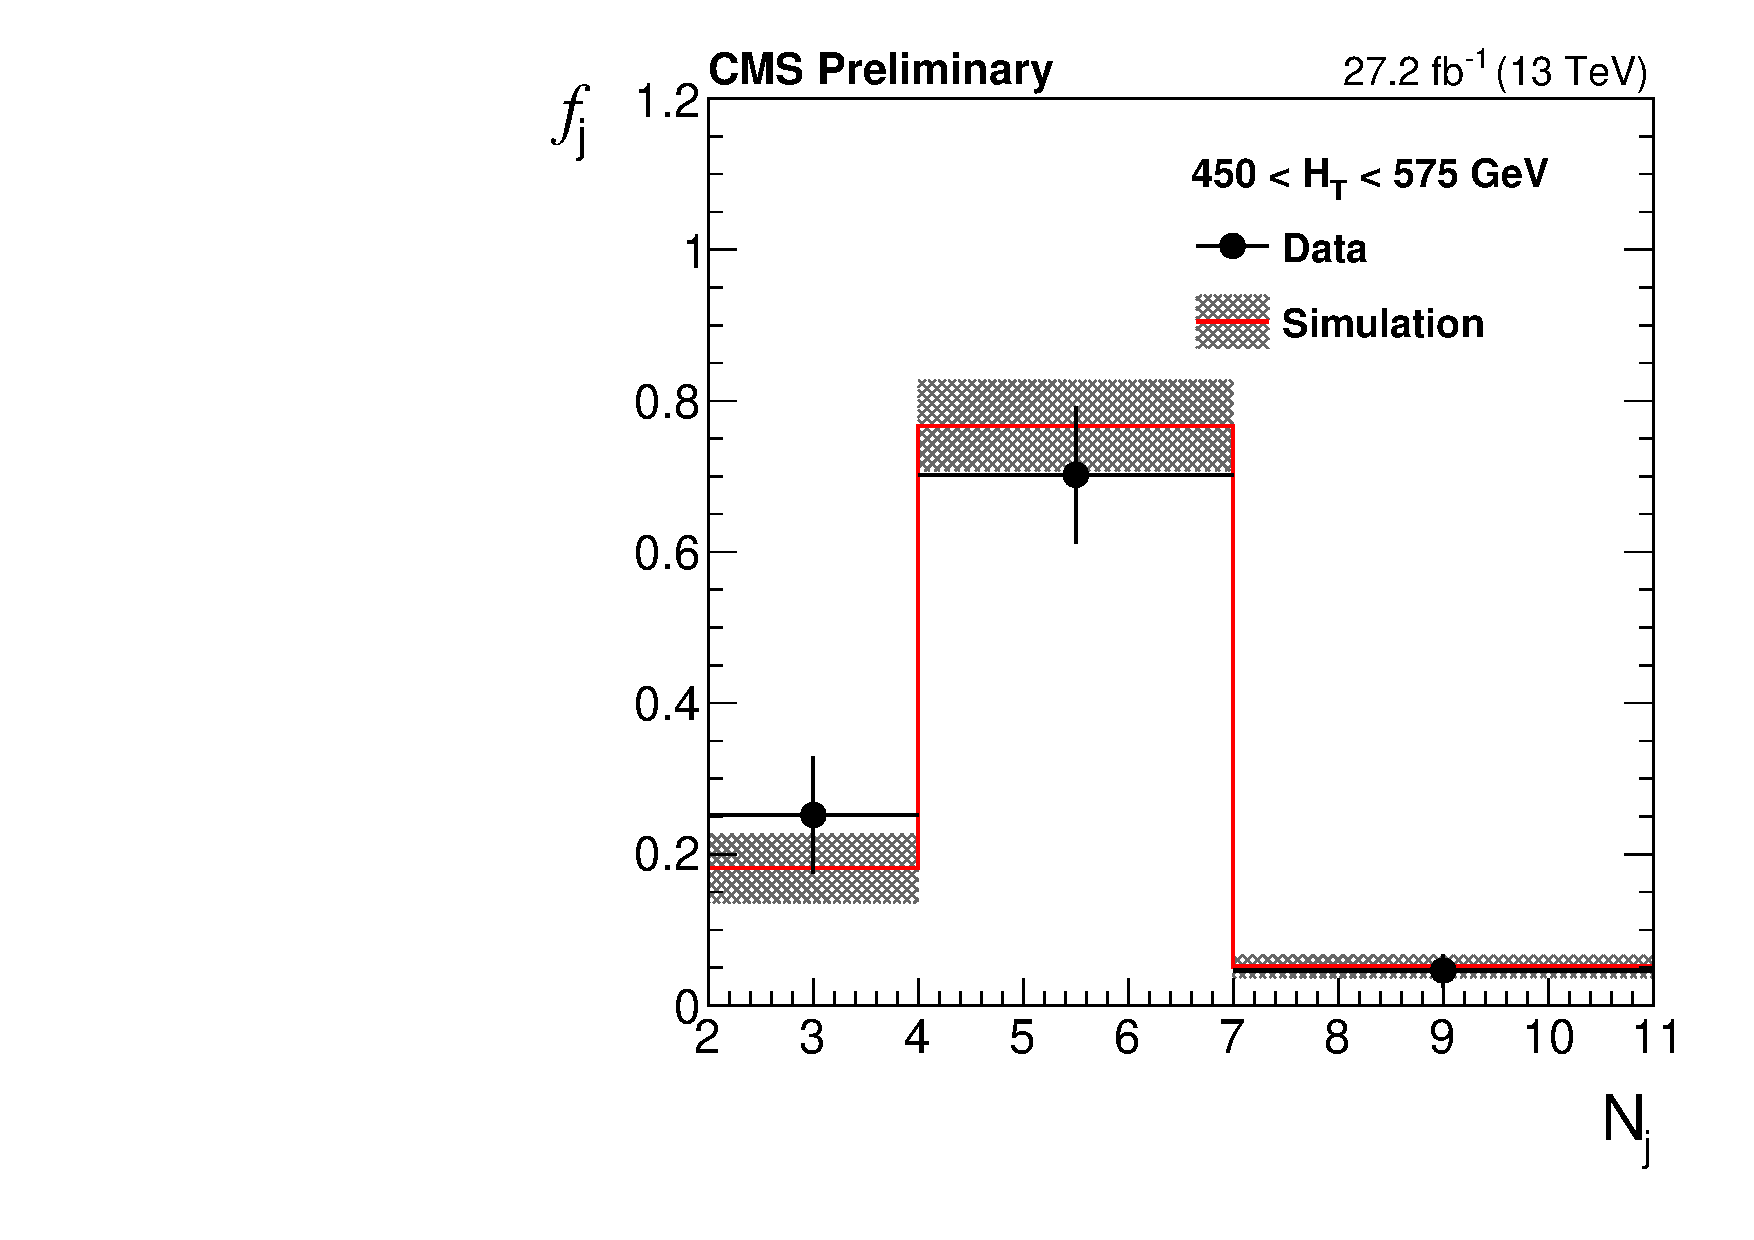
\includegraphics[width=0.35\textwidth]{backgrounds/figs/f_jets_HT450to575_j2toInf_b0toInf}
	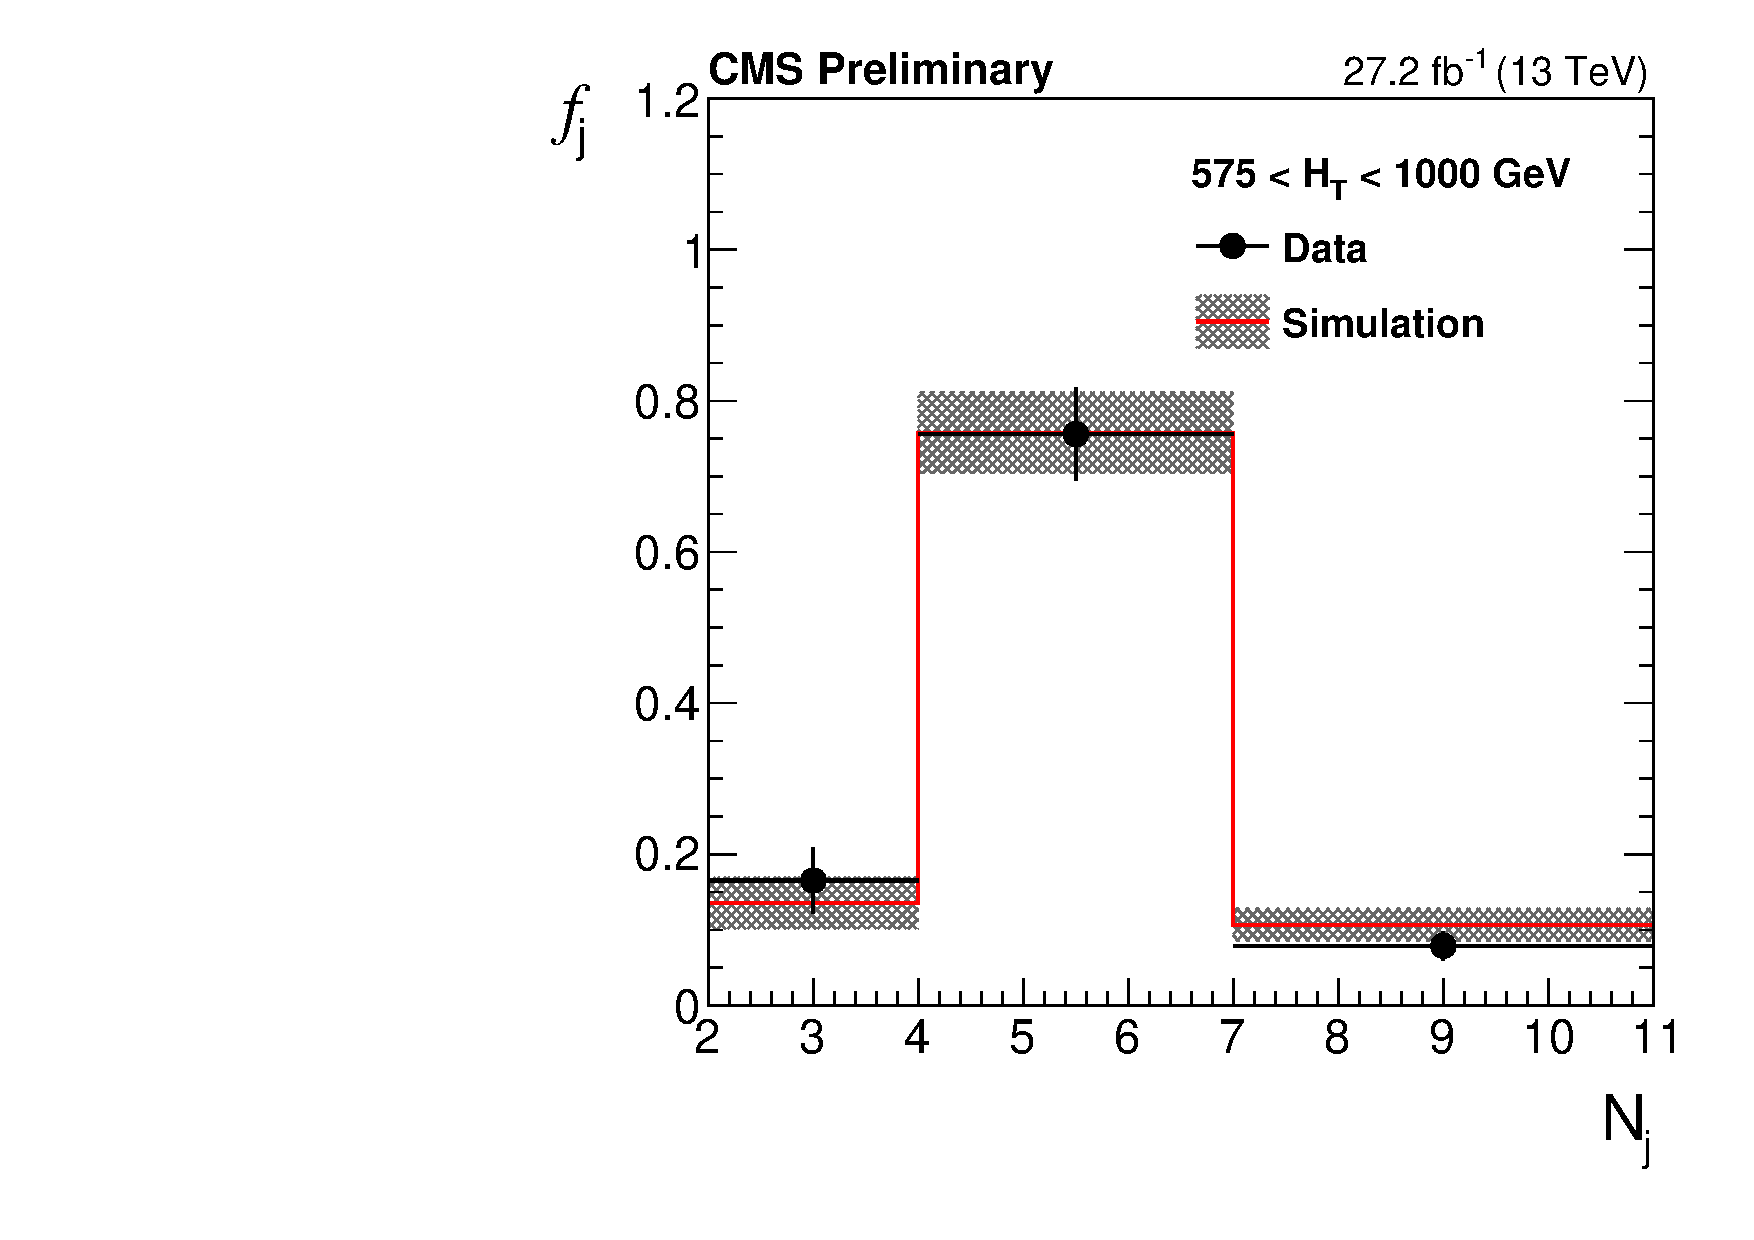
\includegraphics[width=0.35\textwidth]{backgrounds/figs/f_jets_HT575to1000_j2toInf_b0toInf}
	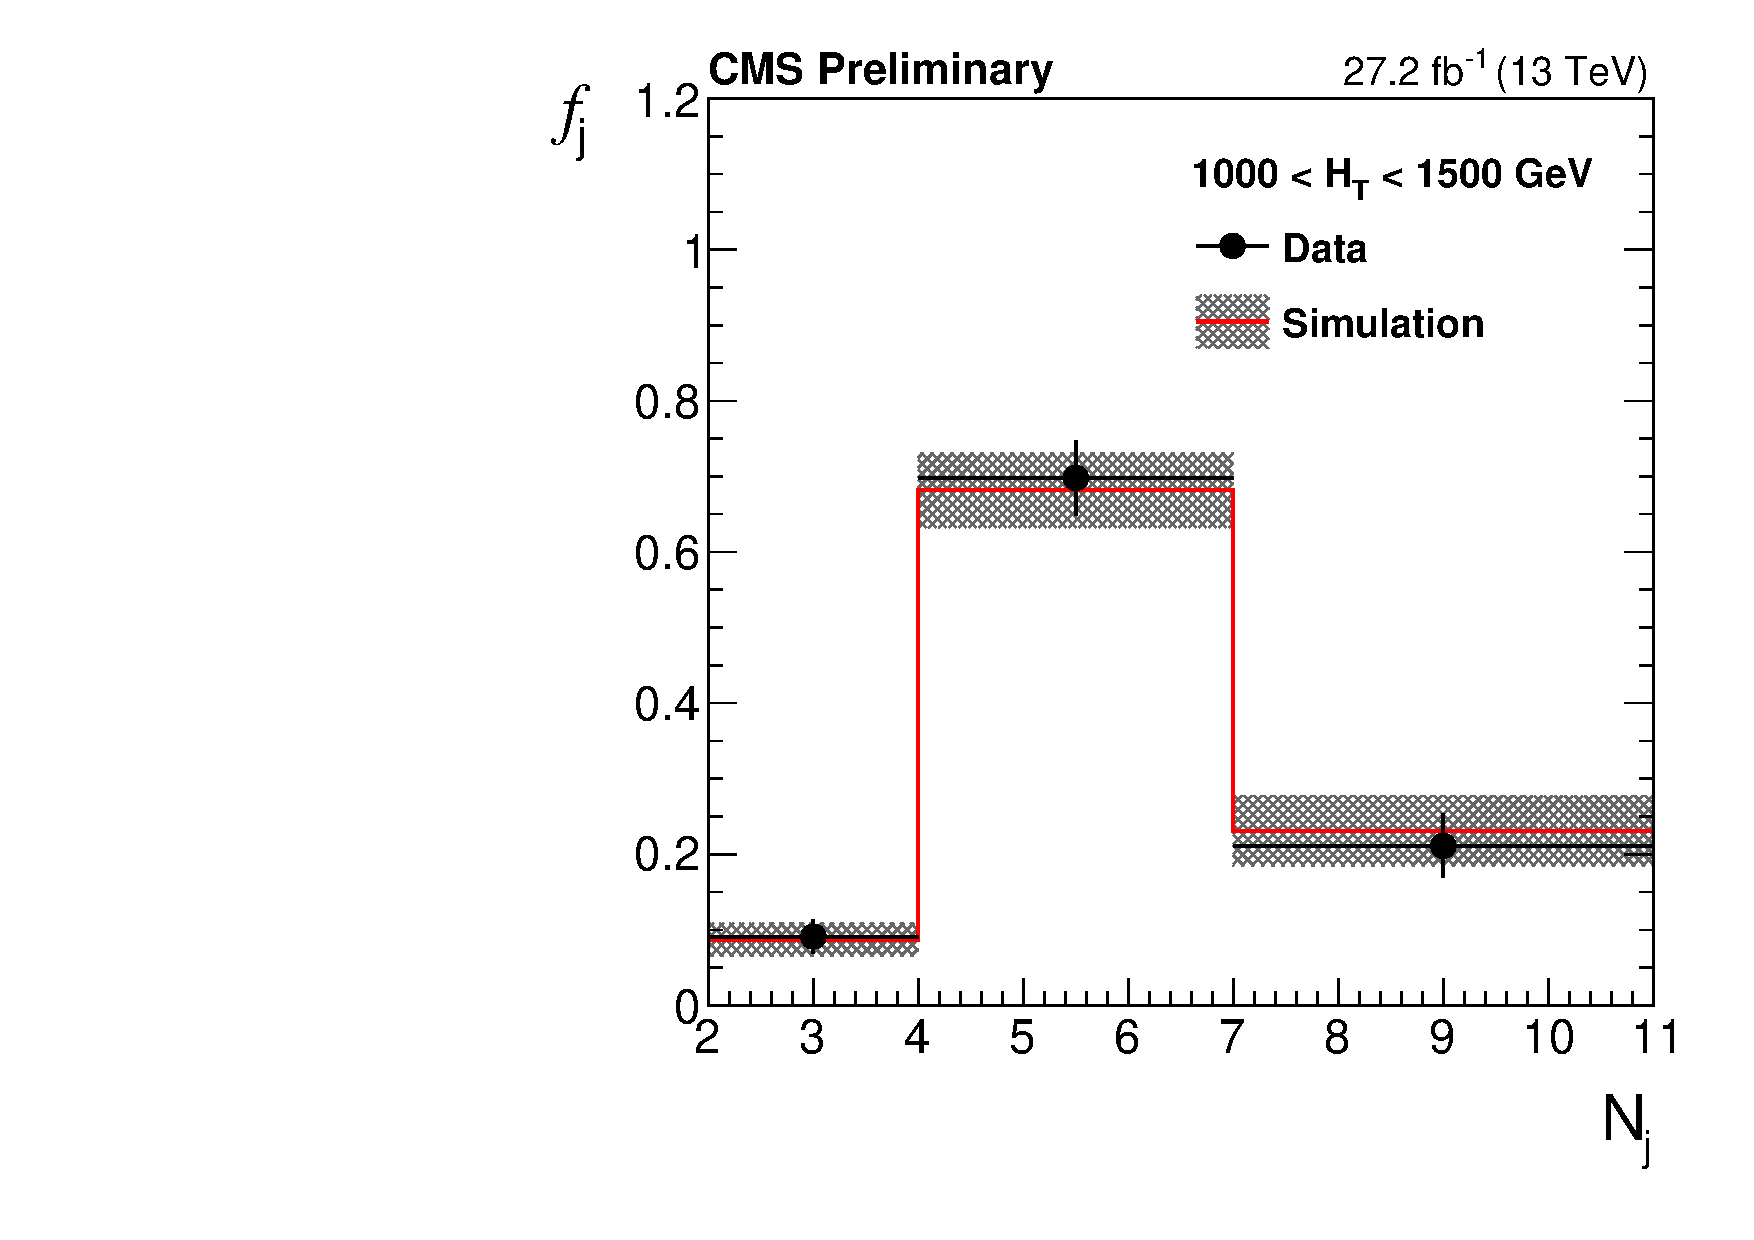
\includegraphics[width=0.35\textwidth]{backgrounds/figs/f_jets_HT1000to1500_j2toInf_b0toInf}
	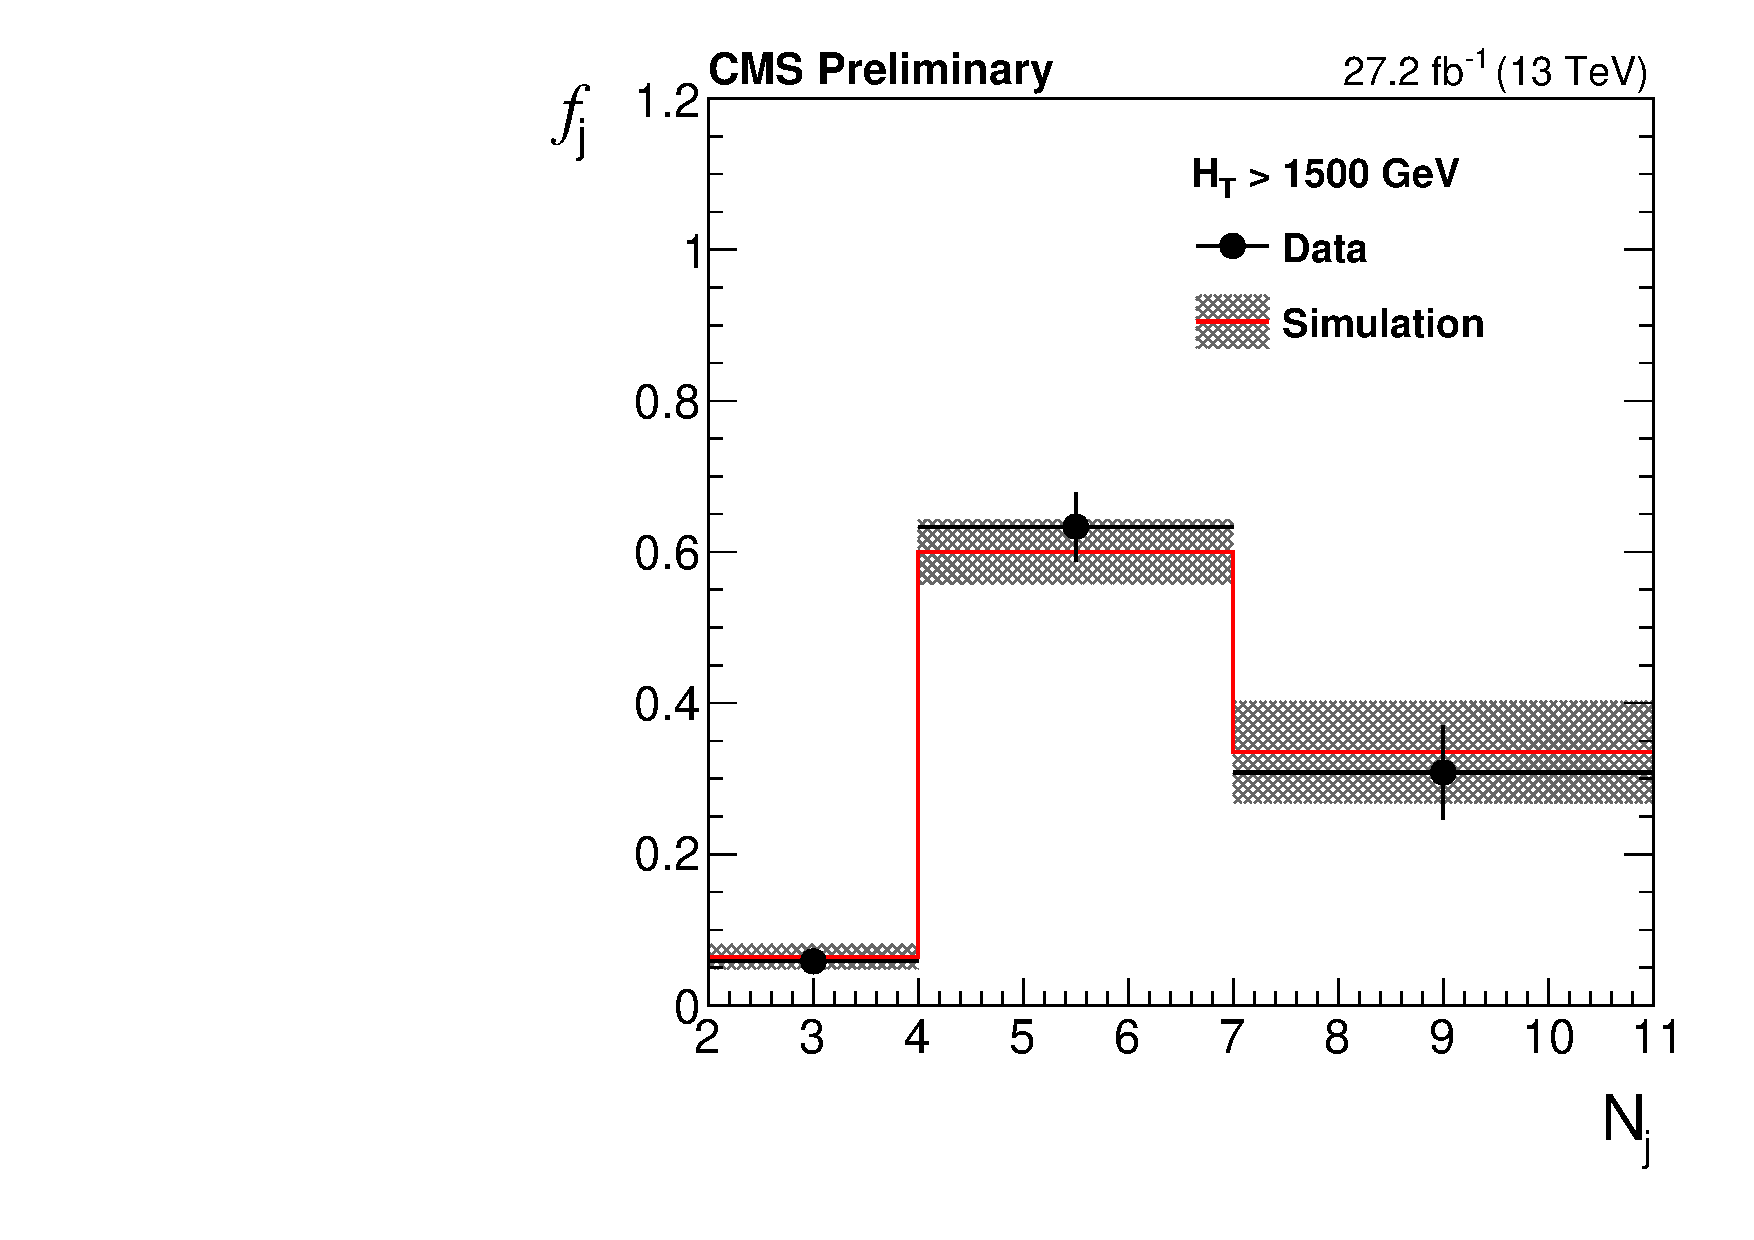
\includegraphics[width=0.35\textwidth]{backgrounds/figs/f_jets_HT1500toInf_j2toInf_b0toInf.pdf}
	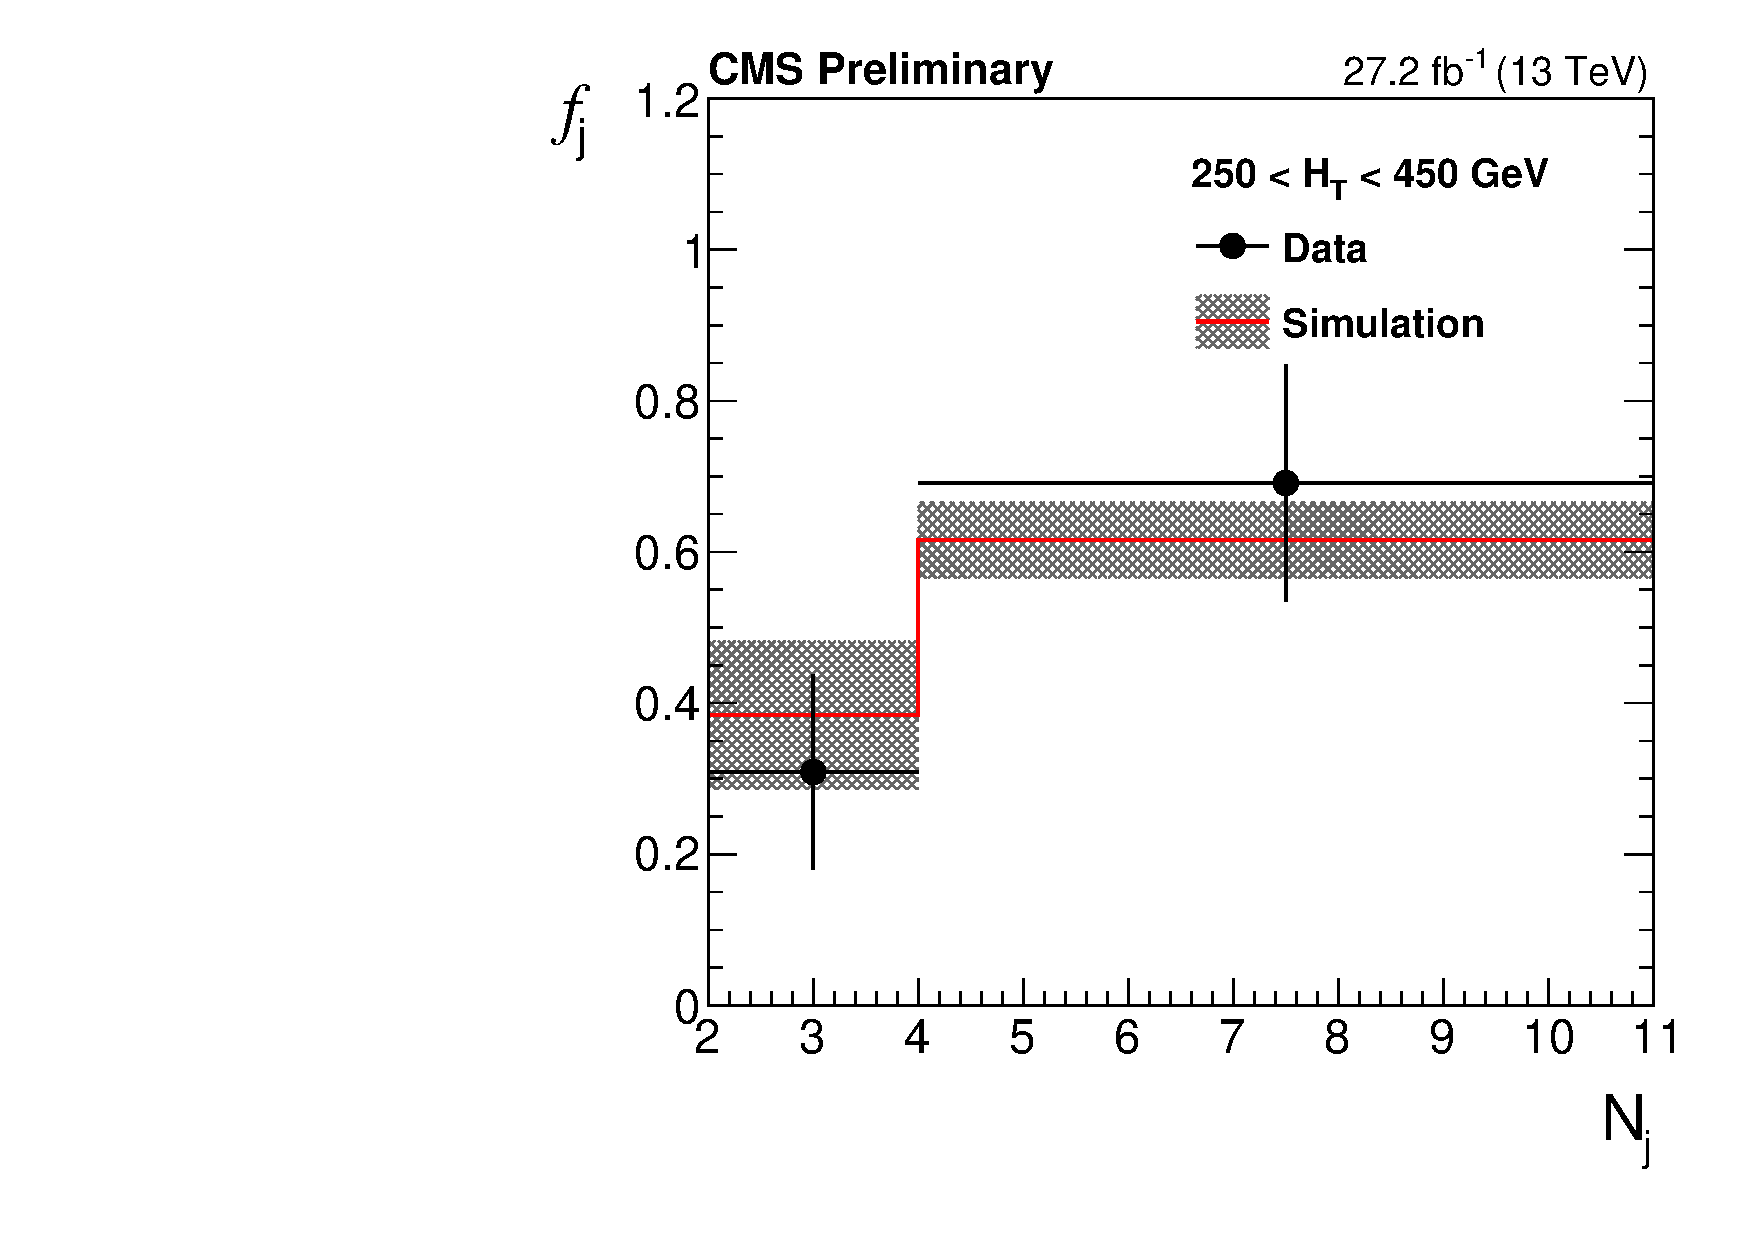
\includegraphics[width=0.35\textwidth]{backgrounds/figs/f_jets_HT250to450_j2toInf_b0toInf}
	\caption{The values of \fj as measured in data in different \HT regions, compared to simulation. The uncertainties include both the statistical error and the systematic sources as listed in table \ref{tbl:fjrbSyst}}
	\label{fig:fj}
\end{figure}
\begin{figure}
	\centering
	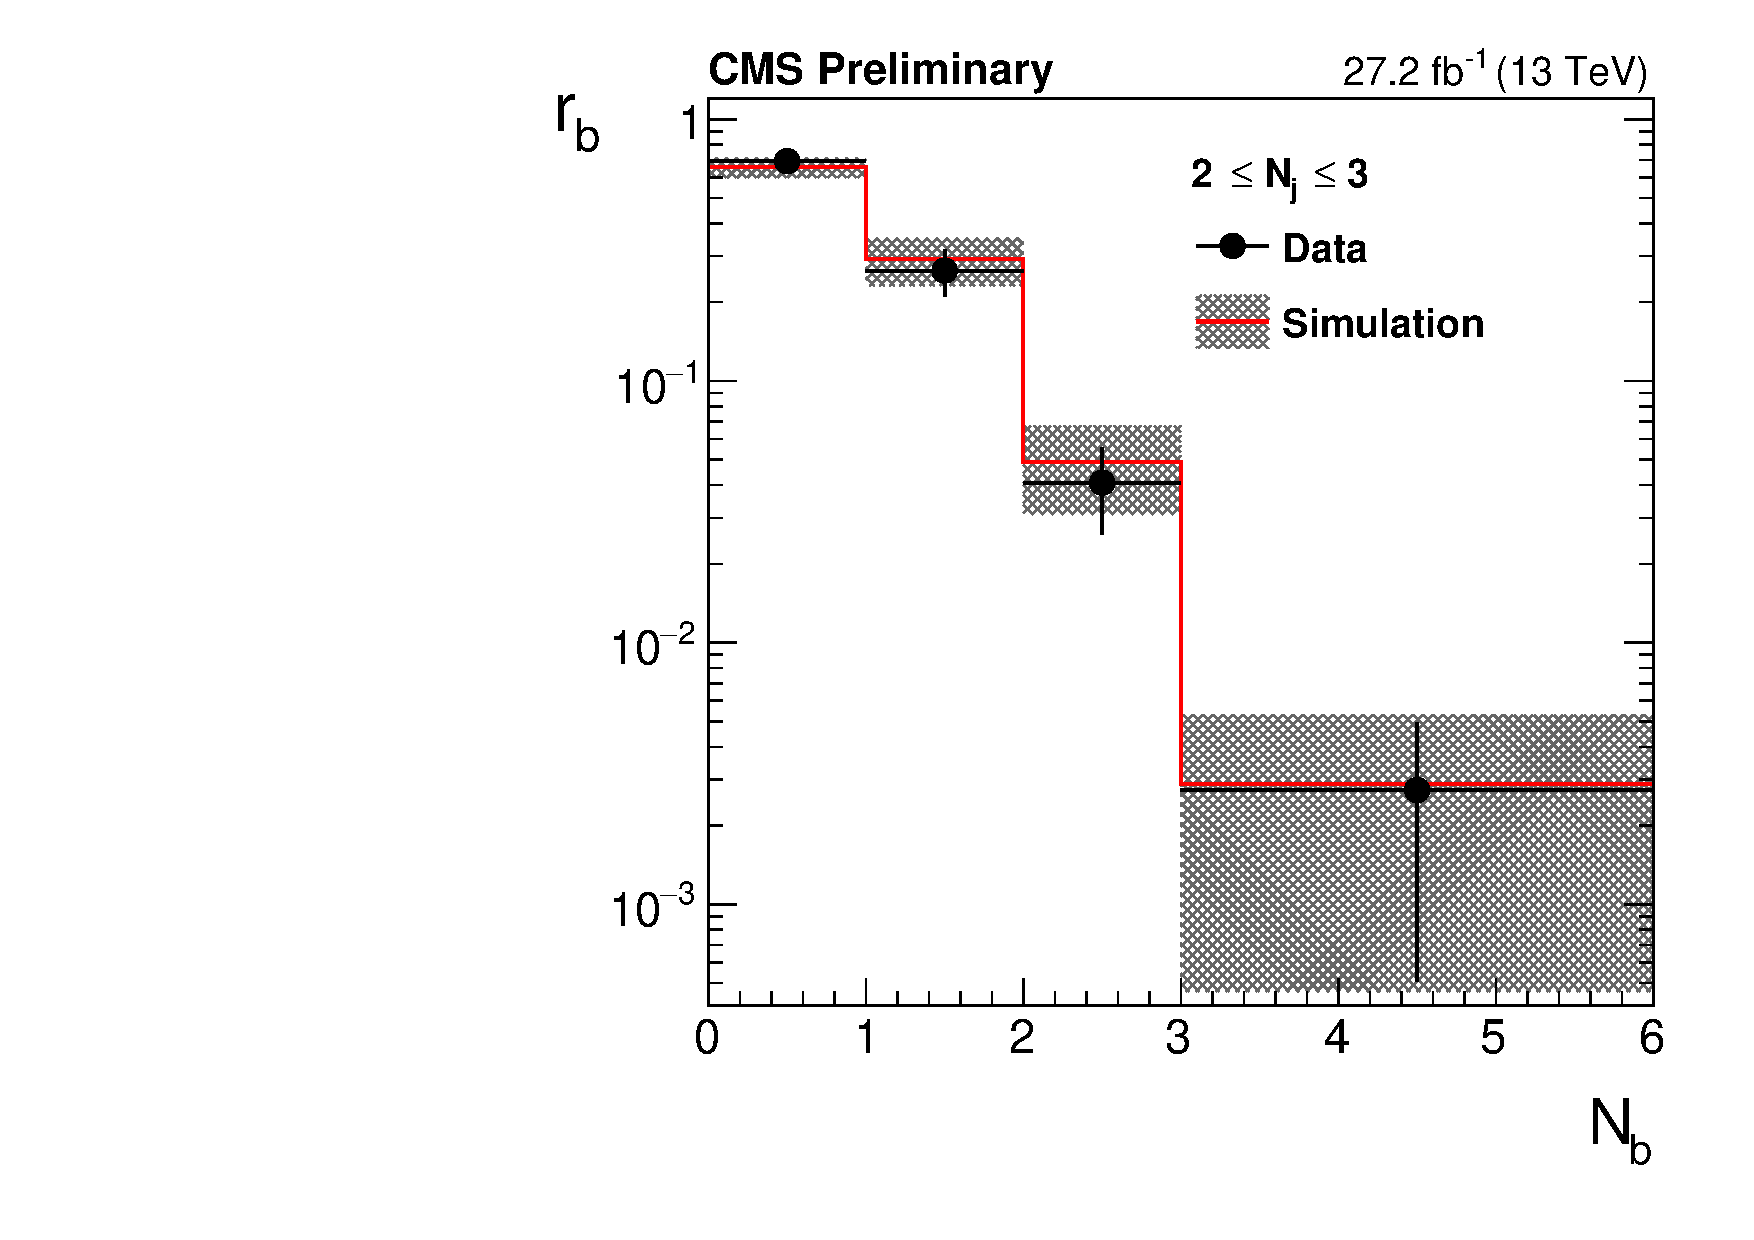
\includegraphics[width=0.45\textwidth]{backgrounds/figs/r_hat_HT250toInf_j2to3_b0toInf}
	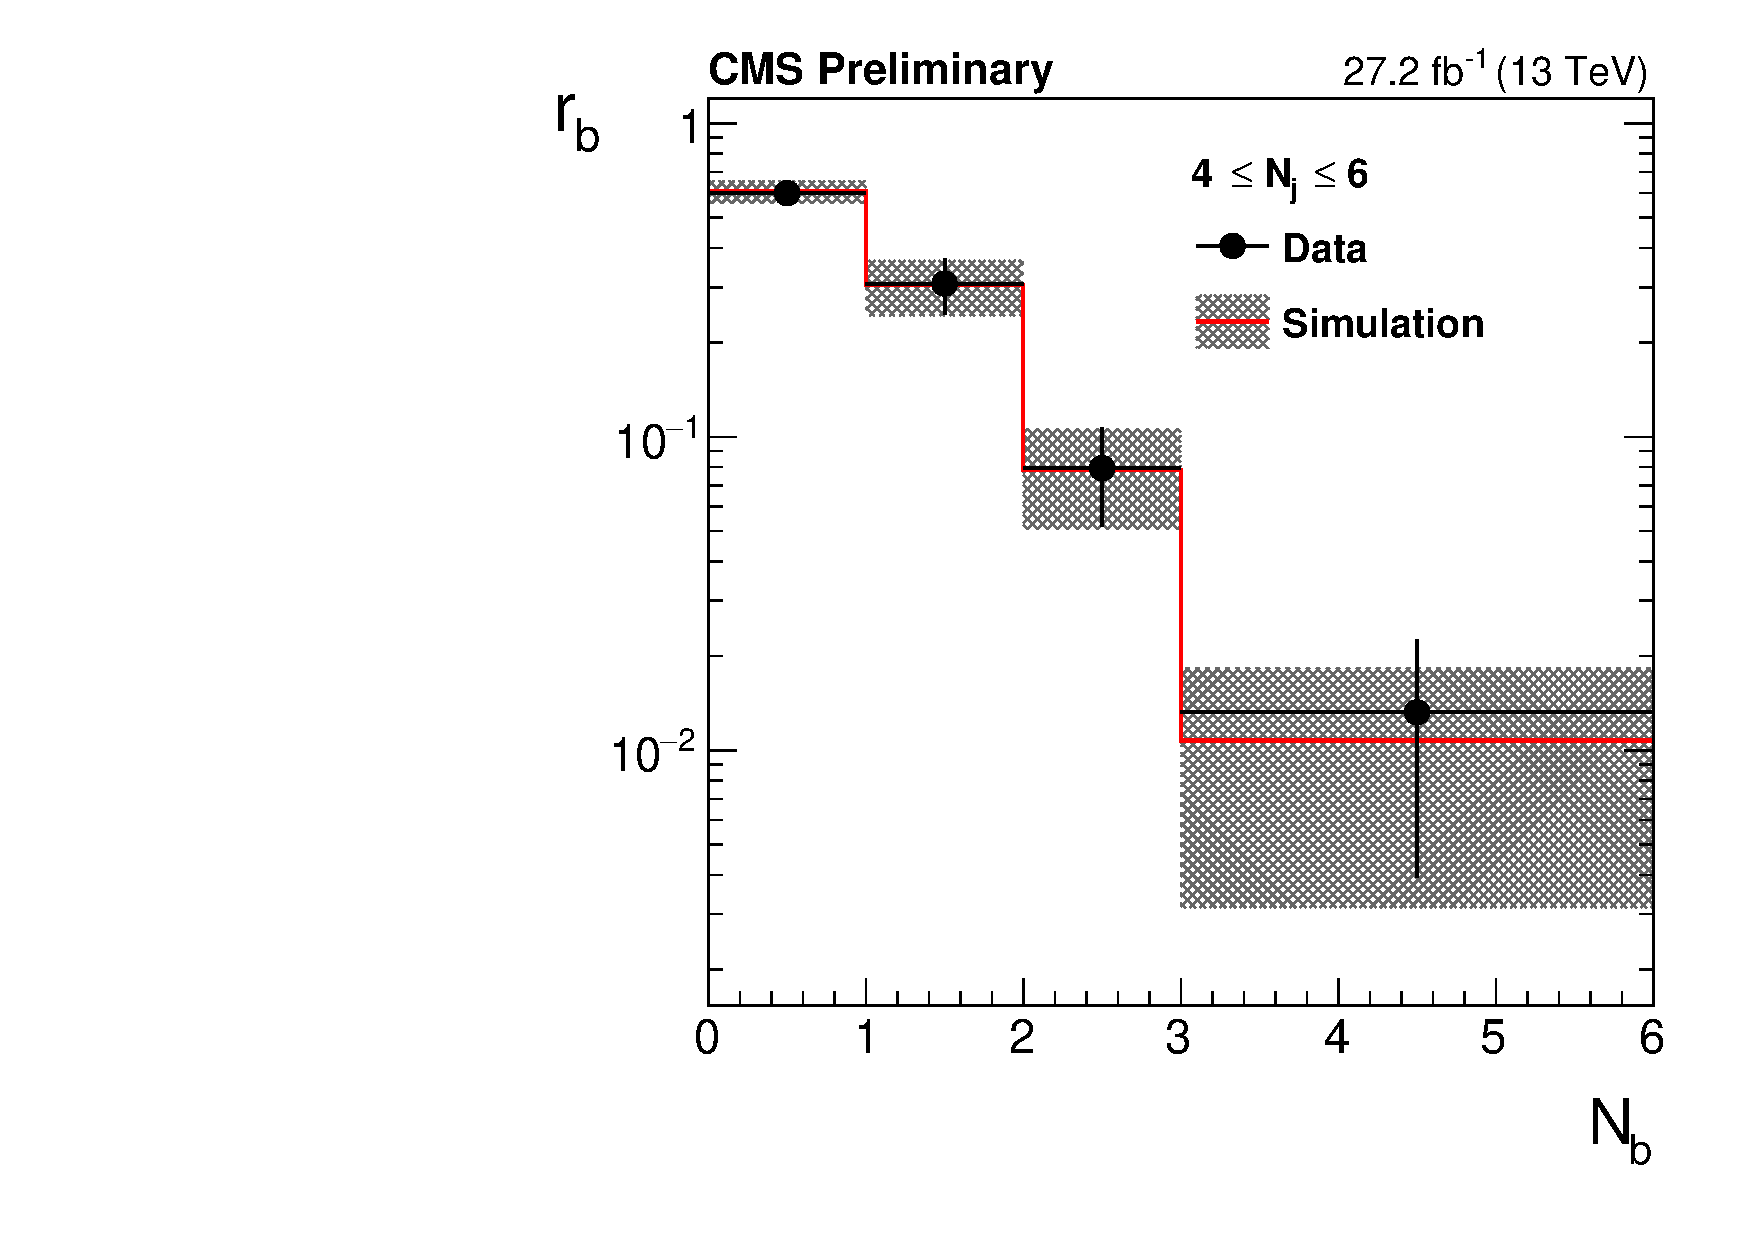
\includegraphics[width=0.45\textwidth]{backgrounds/figs/r_hat_HT250toInf_j4to6_b0toInf}
	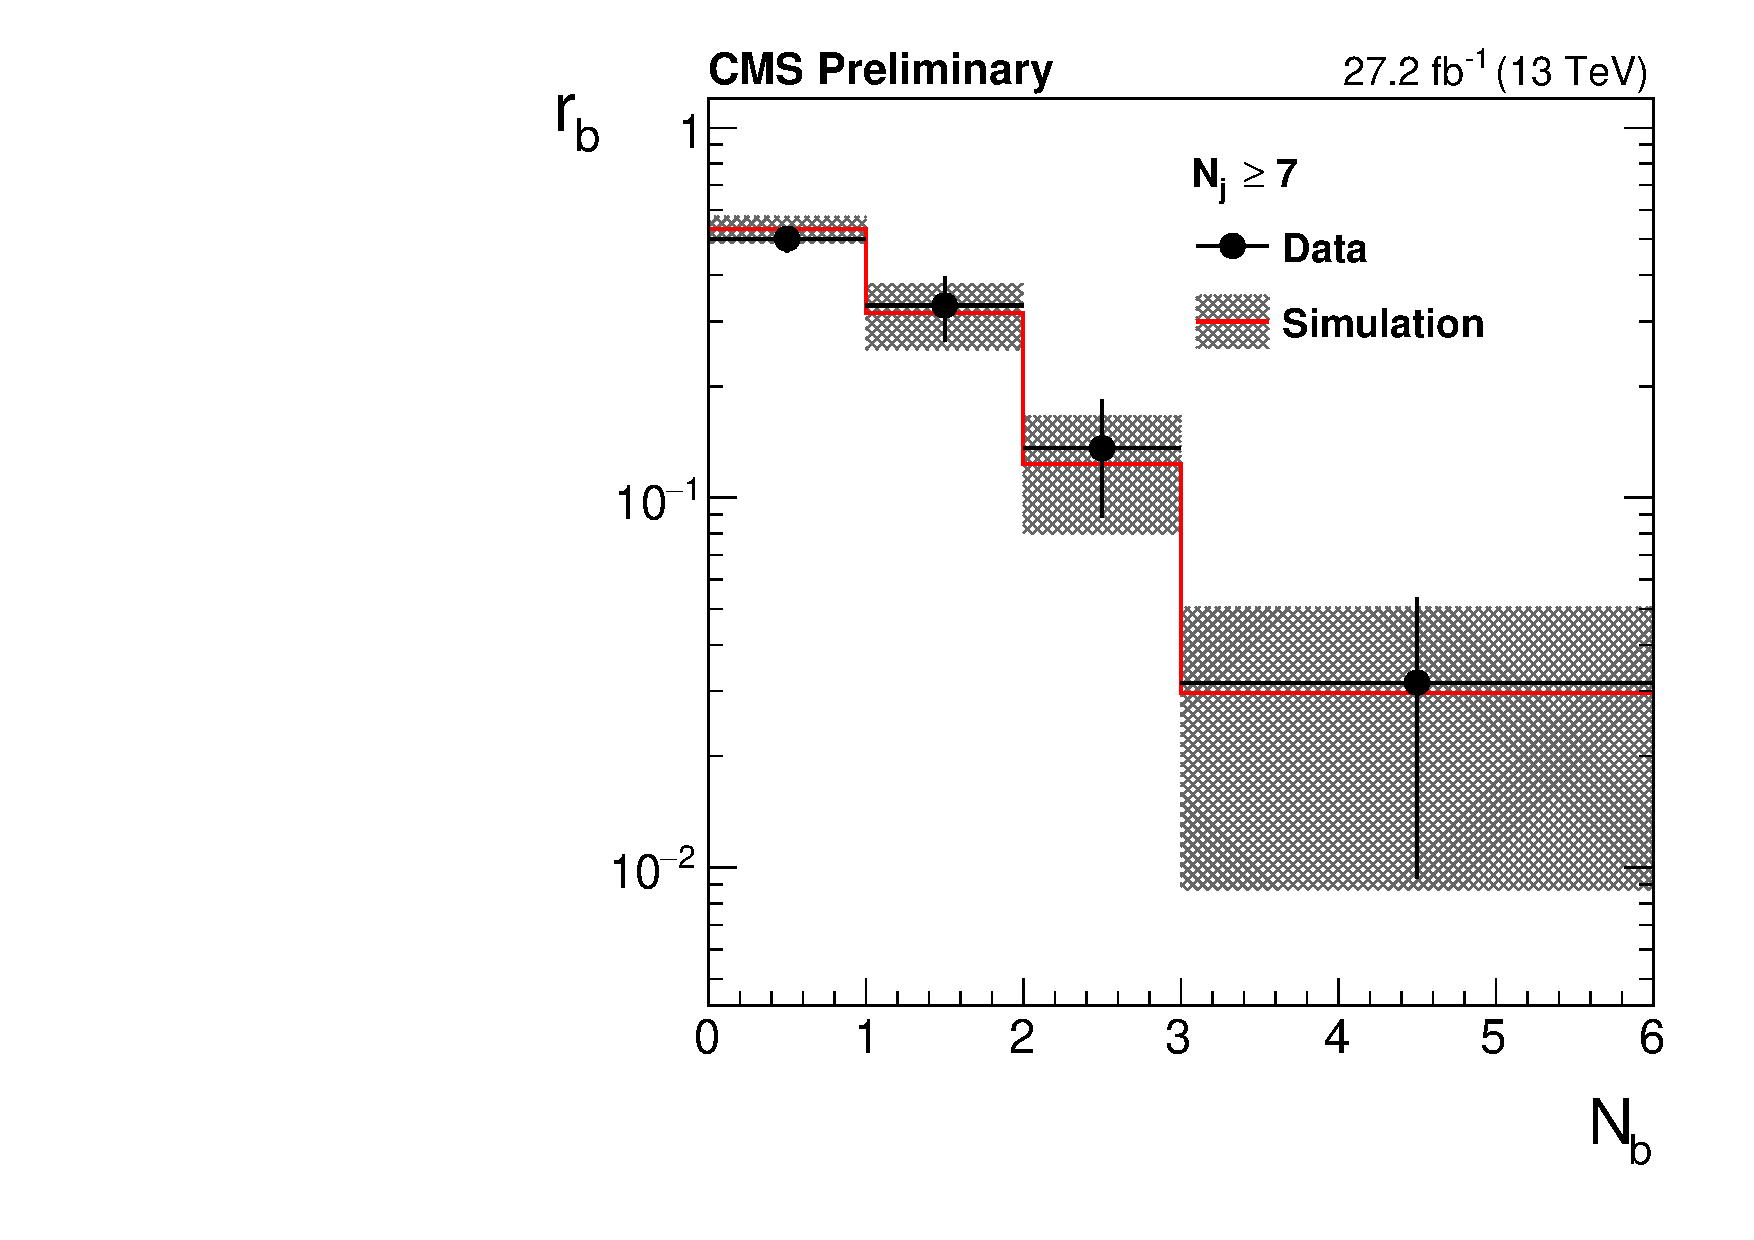
\includegraphics[width=0.45\textwidth]{backgrounds/figs/r_hat_HT250toInf_j7toInf_b0toInf}
	\caption{The values of \rb as measured in data in different \nj regions, compared to simulation. The uncertainties include both the statistical error and the systematic sources as listed in table \ref{tbl:fjrbSyst}}
	\label{fig:rb}
\end{figure}
\begin{table}
	\centering
	 \begin{tabular}{c|ccc|cccc}
      \hline\hline
Observable    & $f_{23}$ & $f_{46}$ & $f_{7^+}$ & $ r_{0}$ & $ r_{1}$ & $ r_{2}$ & $ r_{3+}$\\\hline
Syst. Error   &  25\%   &   7\%   &   20\%   &    8\%       &     20\%     &     35\%    &    70\%      \\ 
\hline\hline
       \end{tabular}
	\caption{Relative uncertainty of \fj and \rb associated with the assumed invariance with respect to \mttwo and \dphi (and \HT for \rb).}
	\label{tbl:fjrbSyst}
\end{table}


\subsection{Monojet Signal Region Prediction}
\label{subsec:qcdMonojet}
The multijet background in control regions with a single jet cannot be estimated using the \dphi technique since \MET is usually very similar to the \HT in these events and typically anti-aligned with the jet. As outlined in section \ref{subsec:multijetCR}, a separate control region is devised which instead selects dijet events that are orthogonal to the multijet signal regions because of an inverted \dphilong cut (and orthogonal to the the monojet SR with the presence of multiple jets). 

The sub-leading jet momentum for in this CR can be seen in figure \ref{fig:subleadingJetPt}. Because jets with \pt below 30\GeV are not considered, monojet events can be classified as those with $p_{\mathrm{T}}^{\mathrm{jet2}} < 30\GeV$, and the CR is used to extrapolate into the regime where $p_{\mathrm{T}}^{\mathrm{jet2}}$ is small. With decreasing $p_{\mathrm{T}}^{\mathrm{jet2}}$, events appear more imbalanced and approximate the topology of a true monojet event, as depicted in figure \ref{fig:monojetCartoon}.
\begin{figure}
	\centering
	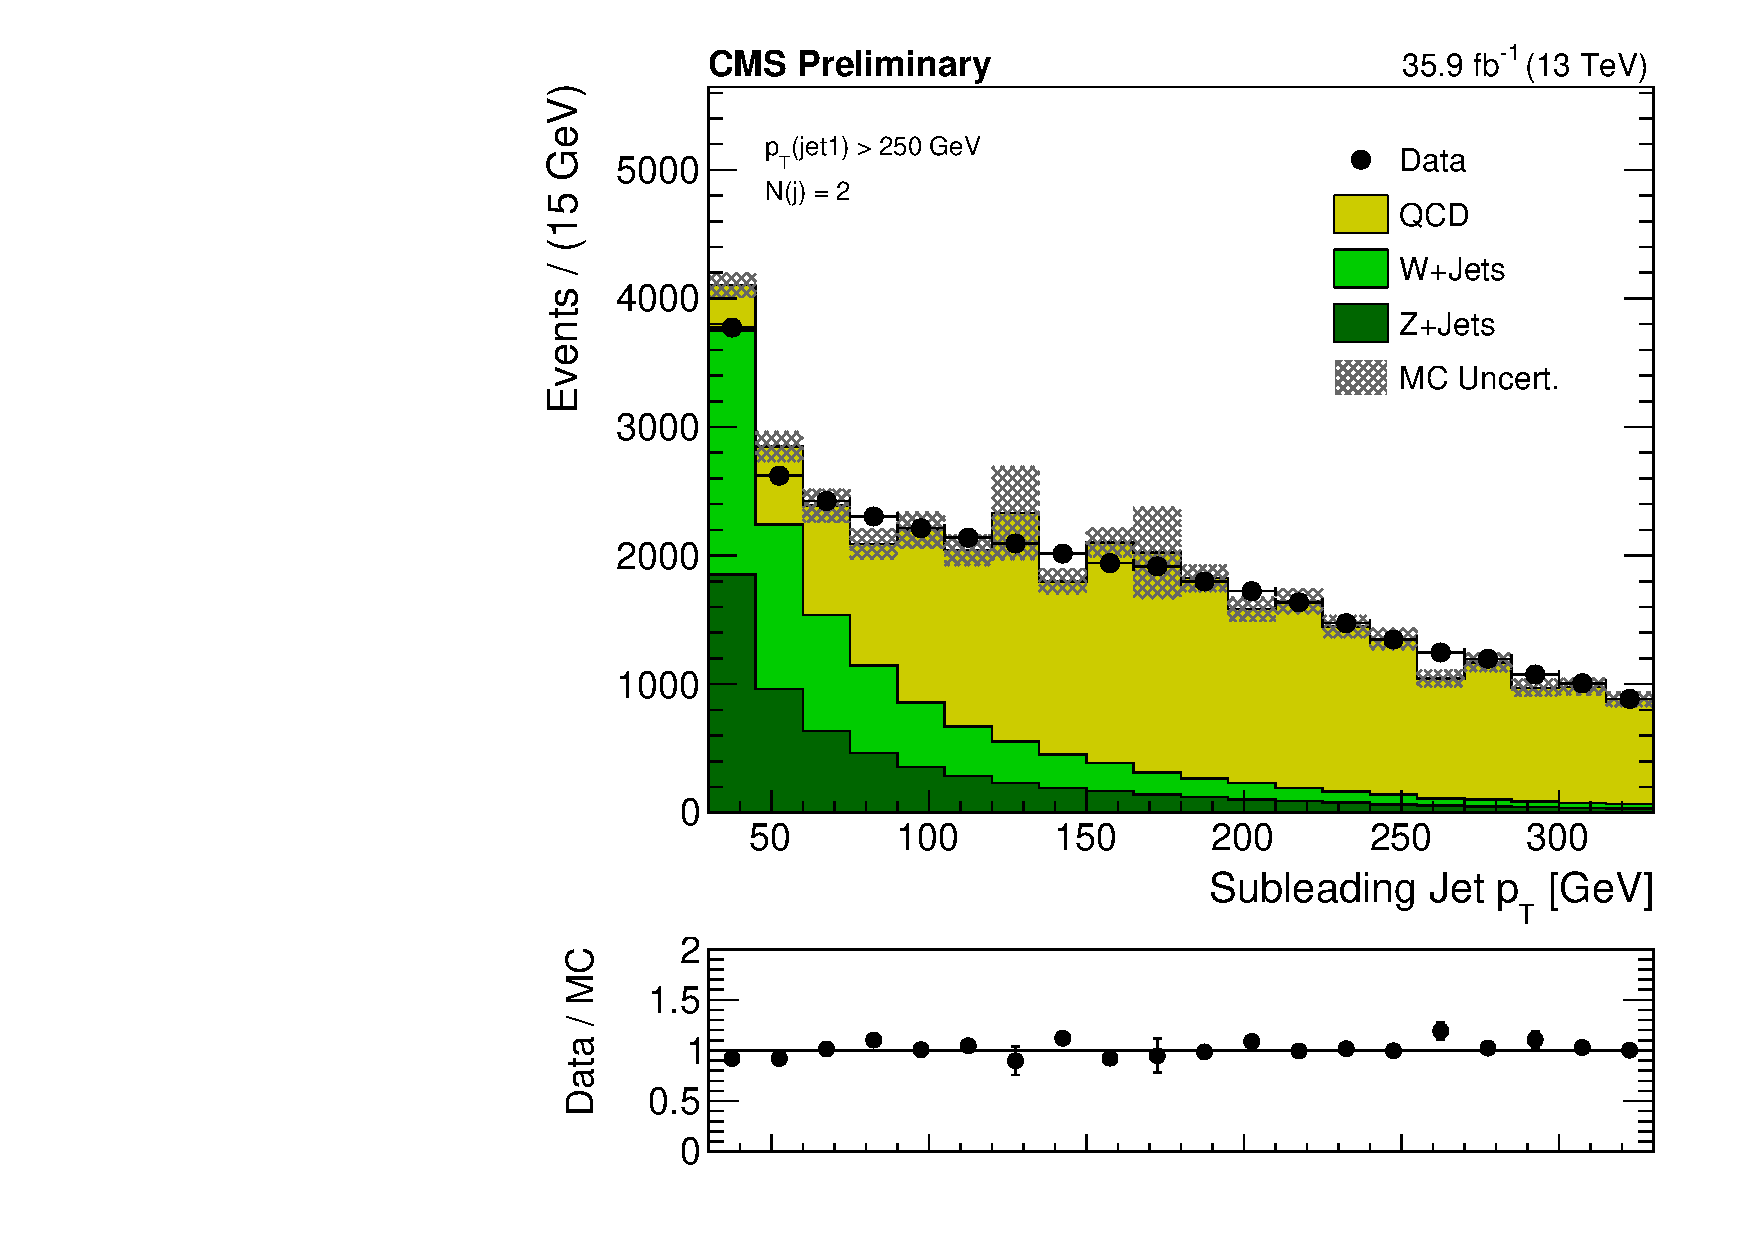
\includegraphics[width=0.45\textwidth]{backgrounds/figs/jet2_pt_35p9ifb}
	\caption{The transverse momentum of the sub-leading jet for dijet events in the monojet QCD background control region. The total yield of the simulation is normalized to the overall yield in data.}
	\label{fig:subleadingJetPt}
\end{figure}
\begin{figure}
	\centering
	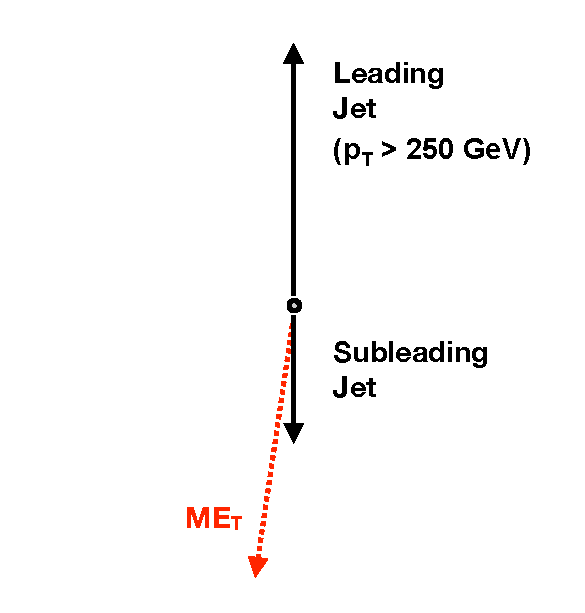
\includegraphics[width=0.45\textwidth]{backgrounds/figs/dijet_cartoon_Moriond2017}
	\caption{An illustration of ``unbalanced'' dijet events. As the momentum of the sub-leading jet decreases, \MET is more anti-aligned with the primary jet and approaches the topology of a monojet event.}
	\label{fig:monojetCartoon}
\end{figure}

The predicted yield of multijet background in a monojet $p_{\mathrm{T}}^{\mathrm{jet1}}$ bin is determined according to equation \ref{eq:monojetEstimate}, where $f_{\mathrm{QCD}}$ is the fraction of QCD events as measured in the region with $30 < p_{\mathrm{T}}^{\mathrm{jet2}} < 60 \GeV$ and $N_{\mathrm{data}}$ is the yield in data of dijet events with $30 < p_{\mathrm{T}}^{\mathrm{jet2}} < 60 \GeV$. Assuming $N_{\mathrm{data}}(0-30) < N_{\mathrm{data}}(30-60)$, this estimate provides an upper bound on the total multijet background contribution in each monojet CR. A systematic uncertainty of 50\% on the QCD fraction $f_{\mathrm{QCD}}$ is assigned as a conservative estimate.
\begin{equation}
	N_{\mathrm{QCD}}(p_{\mathrm{T}}^{\mathrm{jet1}}) = N_{\mathrm{data}}(30-60,p_{\mathrm{T}}^{\mathrm{jet1}}) \cdot f_{\mathrm{QCD}}(30-60,p_{\mathrm{T}}^{\mathrm{jet1}})
	\label{eq:monojetEstimate}
\end{equation}

% --------------------------------------------------------------------------- %
% --------------------------------------------------------------------------- %
